\clearpage
\subsubsection{Exit} % (fold)
\label{sub:exit}

The exit statement, or the return in C, ends the current \nameref{sub:function} or \nameref{sub:procedure}. This is useful for skipping the rest of the processing of the Function or Procedure, exiting it early and returning to the calling code. 

\begin{figure}[h]
   \centering
   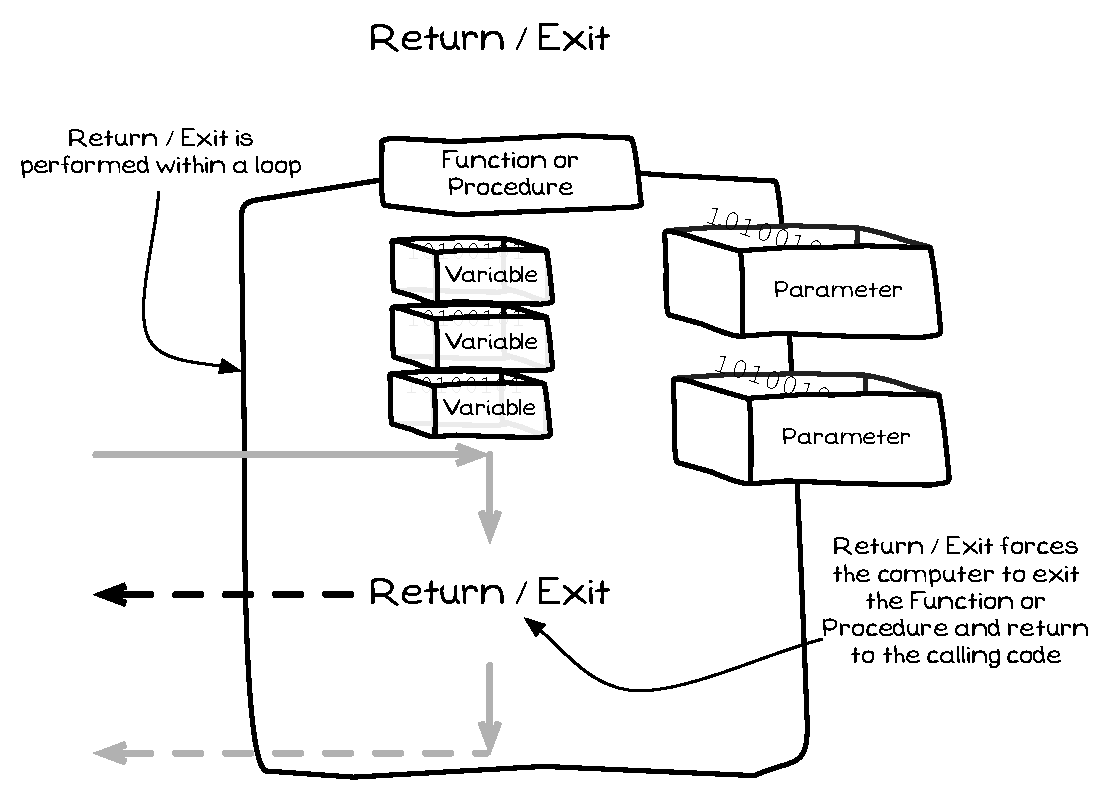
\includegraphics[width=\textwidth]{./topics/control-flow/diagrams/Return} 
   \caption{Exit ends the current Function or Procedure}
   \label{fig:exit}
\end{figure}

\mynote{
\begin{itemize}
  \item Exit is an \textbf{action}, allowing you to jump out of the current Function or Procedure, and return to the calling code.
  \item The Exit should be coded within a \nameref{sub:branching} statement that checks if the Function or Procedure should end.
\end{itemize}
}

\csection{C's version of the exit statement is the \nameref{sub:return_statement}. The return statement also provides the value that will be returned when exiting from a Function. As this sets the value to be returned you must have a return statement as the last action within a Function.}

% subsection return_or_exit_statement (end)